\documentclass{book}

\usepackage{amssymb}
\usepackage{amsmath}
\usepackage{amsthm}
\usepackage{arydshln}
\usepackage[dvipsnames]{xcolor}
\usepackage{calc}
\usepackage{cancel}
\usepackage{caption}
\usepackage{cite}
\usepackage{color}
\usepackage{enumitem}
\usepackage{esint}
\usepackage{etoolbox}
\usepackage{float}
\usepackage{framed}
\usepackage{fullpage}
\usepackage{gensymb}
\usepackage[margin=1in]{geometry}
\usepackage{graphicx}
\usepackage{listings}
\usepackage{multirow}
\usepackage{subfiles}
\usepackage{rsfso}
\usepackage{tikz}
\usepackage{tikz-3dplot}
\usepackage{ushort}
\usepackage{wrapfig}
\usepackage{soul}
\usepackage{epstopdf}
\usepackage{array}
\usepackage{slashbox}
\usepackage{pgfplots}

% pdf versions
\pdfoptionpdfminorversion=7

% handle page stretching
\raggedbottom

% Graphics file location
\graphicspath{{Graphics/}{../Graphics/}}

% Use for drawings
\usetikzlibrary{angles,arrows,calc,decorations,intersections,patterns,positioning,quotes,shapes}
\usetikzlibrary{shapes.geometric}
\usetikzlibrary{decorations.pathreplacing}
\newcommand{\midarrow}{\tikz \draw[-latex] (0,0) -- +(.1,0);}

% Tikz commands for drawing block diagrams, etc...
\tikzset{%
	block/.style    = {draw, rectangle, minimum height = 2em, minimum width = 2em},
	sum/.style      = {draw, circle}, % Adder
	input/.style    = {fill=white, rectangle}, % Input
	output/.style   = {fill=white, rectangle}, % Output
	waypoint/.style   = {coordinate}, % Output
}

\tikzset{%
	startstop/.style= {draw, rectangle, rounded corners, minimum width=2cm, minimum height=1cm,text centered},
	inout/.style    = {draw, trapezium, trapezium left angle=70, trapezium right angle=110, minimum width=2cm, minimum height=1cm, text centered},
	process/.style  = {draw, rectangle, minimum width=2cm, minimum height=1cm, text centered},
	decision/.style = {draw, diamond, minimum width=1.5cm, minimum height=1cm, text centered, diamond, aspect=2},
	arrow/.style    = {thick,-latex,>=stealth},		
}

\tikzset{
	saveuse path/.code 2 args={
		\pgfkeysalso{#1/.style={insert path={#2}}}%
		\global\expandafter\let\csname pgfk@\pgfkeyscurrentpath/.@cmd\expandafter\endcsname
		% not optimal as it is now global through out the document
		\csname pgfk@\pgfkeyscurrentpath/.@cmd\endcsname
		\pgfkeysalso{#1}},
	/pgf/math set seed/.code=\pgfmathsetseed{#1}}

% Define Laplace, Fourier transform symbols
\newcommand{\LT}{\mathcal{L}}
\newcommand{\FT}{\mathcal{F}}

% Define adjugate function
\newcommand{\adj}{\text{adj}}

% Define rank function
\newcommand{\rank}{\text{rank}}

% commands to speed up writing j\omega and s-plane
\newcommand{\jw}{j\omega}
\newcommand{\jt}{j\theta}
\newcommand{\wt}{\omega t}
\newcommand{\spl}{s\textrm{-plane}}
\newcommand{\Lm}{\textrm{Lm }}
\newcommand{\logg}{\log_{10}}
% Clean up overline/underline for math mode
\def\obar#1{\bar{#1}}
\def\ubar#1{\ushort{#1}}

\newcommand{\exmp}{\subsubsection*{Example}}
\newcommand{\nib}{\noindent$ \bullet\ $}


\begin{document}
	\section*{Bode Plot Examples}
	Dashed lines show the individual asymptotes. Add these together (and account for the magnitude of the gain and the starting slope/phase due to any integrators) to get the complete sketch.
	\begin{enumerate}
		\item Draw the Bode asymptote plot for 
		\[ G(s) = \dfrac{1}{s(s+2)(s+4)} \]
		\textbf{Solution:} 
		\begin{itemize}
			\item 1 integrator, so start with $ -20 $dB/dec slope with 0dB at $ \omega=1 $ rad/s and $ -90^\circ $ phase.
			\item $ K=\dfrac{1}{2\cdot4} = -18 $ dB, so shift by -18dB (no change to phase plot).
			\item Pole at $ s=-2 $ (blue) add $ -20 $dbB/dec at $ \omega=2 $, and a $ -90^\circ $ shift from $ \omega=0.2 $ to $ \omega=20 $. (Or, adds $ -45^\circ $/dec at $ \omega=0.2 $ and $ +45^\circ $/dec at $ \omega=20 $.)
			\item Pole at $ s=-4 $ (red) add -20dbB/dec at $ \omega=4 $, and a $ -90^\circ $ shift from $ \omega=0.4 $ to $ \omega=40 $. (Or, adds $ -45^\circ $/dec at $ \omega=0.4 $ and $ +45^\circ $/dec at $ \omega=40 $.)
		\end{itemize}
		\begin{center}
			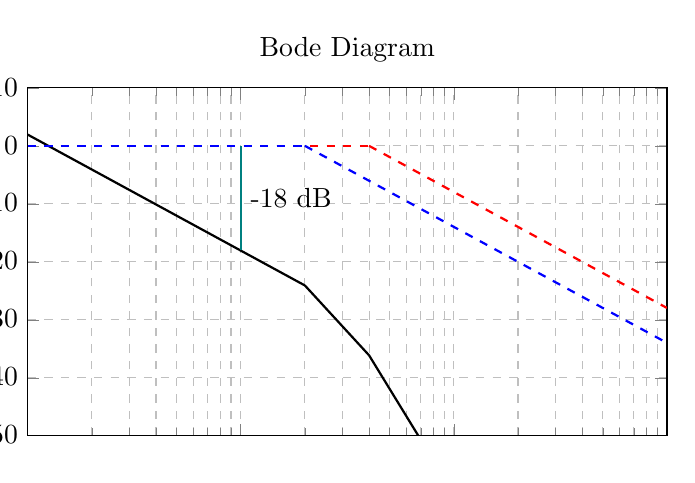
\begin{tikzpicture}[trim axis left,trim axis right]
			\begin{semilogxaxis}[title=Bode Diagram, ylabel=Gain, xmin=1e-1, xmax=1e2, ymin=-50, ymax=10, xticklabels={,,}, width=0.8\textwidth,height=6cm,ytick={-50,-40,-30,-20,-10,0,10},grid=both,grid style={dashed}];	
			\addplot[thick,domain=1e-1:2] {20*log10(1/8)-20*log10(x)};
			\addplot[thick,domain=2:4] {20*log10(1/8)-40*log10(x)+20*log10(2)};
			\addplot[thick,domain=4:1e2] {20*log10(1/8)-60*log10(x)+20*log10(2)+20*log10(4)};
			
			\addplot[teal,thick] coordinates {(1,-18) (1,0)};
			\node[right] at (axis cs: 1,-9) {-18 dB};
			
			\addplot[dashed,thick,domain=1e-1:4,red] {0};
			\addplot[dashed,thick,domain=1e-1:2,blue] {0};
			\addplot[dashed,thick,domain=2:1e2,blue] {20*log10(2)-20*log10(x)};		 
			\addplot[dashed,thick,domain=4:1e2,red] {20*log10(4)-20*log10(x)};		
			\end{semilogxaxis}
			\end{tikzpicture}
			
			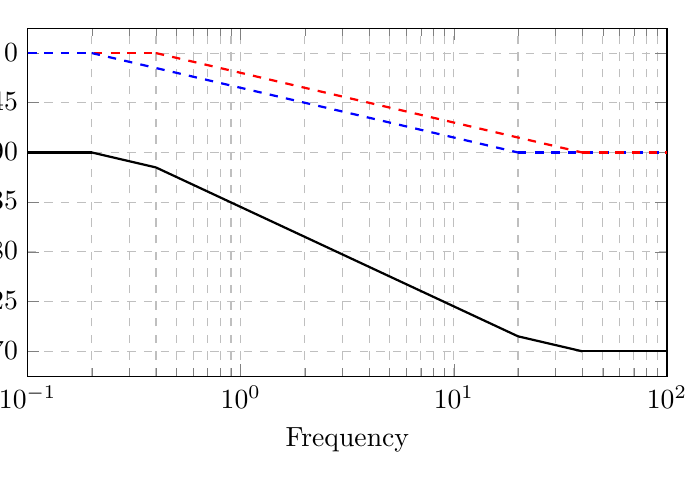
\begin{tikzpicture}[trim axis left,trim axis right]
			\begin{semilogxaxis}[xlabel=Frequency, ylabel=Phase, xmin=1e-1, xmax=1e2, ymin=-292.5, ymax=22.5, width=0.8\textwidth,height=6cm,ytick={-270,-225,-180,-135,-90,-45,0},grid=both,grid style={dashed}];
			
			\addplot[thick,domain=1e-1:0.2] {-90};
			\addplot[thick,domain=0.2:0.4] {-90-45*log10(x)+45*log10(0.2)};
			\addplot[thick,domain=0.4:20] {-90-90*log10(x)+45*log10(0.2)+45*log10(0.4)};
			\addplot[thick,domain=20:40] {-90-45*log10(x)+45*log10(0.2)+45*log10(0.4)-45*log10(20)};
			\addplot[thick,domain=40:1e2] {-270};
			
			\addplot[dashed,thick,domain=1e-1:0.4,red] {0};
			\addplot[dashed,thick,domain=1e-1:0.2,blue] {0};
			\addplot[dashed,thick,domain=20:1e2,blue] {-90};
			\addplot[dashed,thick,domain=40:1e2,red] {-90};
			\addplot[dashed,thick,domain=0.2:20,blue] {-45*log10(x)+45*log10(0.2)};		 
			\addplot[dashed,thick,domain=0.4:40,red] {-45*log10(x)+45*log10(0.4)};	
			
			\end{semilogxaxis}
			\end{tikzpicture}
		\end{center}
	\clearpage
		\item Draw the Bode asymptote plot for 
		\[ G(s) = \dfrac{(s+5)}{(s+2)(s+4)} \]
		\textbf{Solution:}
		\begin{itemize}
			\item No integrators, so start with a flat line on $ 0 $dB and $ 0^\circ $ phase.
			\item $ K=\dfrac{5}{2\cdot4} = -4 $ dB, so shift by -4dB (no change to phase plot).
			\item Pole at $ s=-2 $ (blue) add $ -20 $dbB/dec at $ \omega=2 $, and a $ -90^\circ $ shift from $ \omega=0.2 $ to $ \omega=20 $. (Or, adds $ -45^\circ $/dec at $ \omega=0.2 $ and $ +45^\circ $/dec at $ \omega=20 $.)
			\item Pole at $ s=-4 $ (red) add -20dbB/dec at $ \omega=4 $, and a $ -90^\circ $ shift from $ \omega=0.4 $ to $ \omega=40 $. (Or, adds $ -45^\circ $/dec at $ \omega=0.4 $ and $ +45^\circ $/dec at $ \omega=40 $.)
			\item Zero at $ s=-5 $ (green) add +20dbB/dec at $ \omega=5 $, and a $ +90^\circ $ shift from $ \omega=0.5 $ to $ \omega=50 $. (Or, adds $ +45^\circ $/dec at $ \omega=0.5 $ and $ -45^\circ $/dec at $ \omega=50 $.)
		\end{itemize}
		\begin{center}
			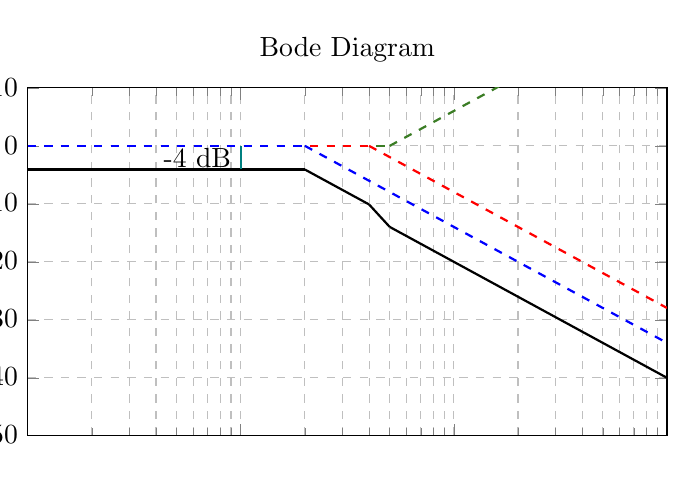
\begin{tikzpicture}[trim axis left,trim axis right]
			\begin{semilogxaxis}[title=Bode Diagram, ylabel=Gain, xmin=1e-1, xmax=1e2, ymin=-50, ymax=10, xticklabels={,,}, width=0.8\textwidth,height=6cm,ytick={-50,-40,-30,-20,-10,0,10},grid=both,grid style={dashed}];	
			\addplot[thick,domain=1e-1:2] {20*log10(5/8)};
			\addplot[thick,domain=2:4] {20*log10(5/8)-20*log10(x)+20*log10(2)};
			\addplot[thick,domain=4:5] {20*log10(5/8)-40*log10(x)+20*log10(2)+20*log10(4)};
			\addplot[thick,domain=5:1e2] {20*log10(5/8)-20*log10(x)+20*log10(2)+20*log10(4)-20*log10(5)};
			
			\addplot[teal,thick] coordinates {(1,-4) (1,0)};
			\node[left] at (axis cs: 1,-2) {-4 dB};
			
			\addplot[dashed,thick,domain=1e-1:5,OliveGreen] {0};
			\addplot[dashed,thick,domain=1e-1:4,red] {0};
			\addplot[dashed,thick,domain=1e-1:2,blue] {0};
			\addplot[dashed,thick,domain=2:1e2,blue] {20*log10(2)-20*log10(x)};		 
			\addplot[dashed,thick,domain=4:1e2,red] {20*log10(4)-20*log10(x)};	 
			\addplot[dashed,thick,domain=5:1e2,OliveGreen] {-20*log10(5)+20*log10(x)};		
			\end{semilogxaxis}
			\end{tikzpicture}
			
			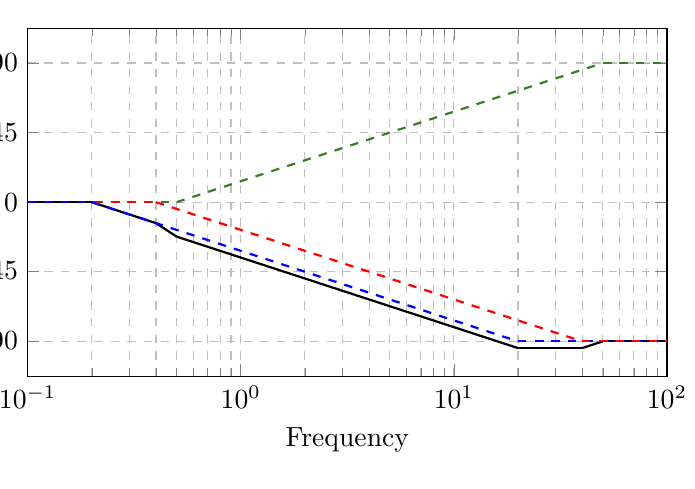
\begin{tikzpicture}[trim axis left,trim axis right]
			\begin{semilogxaxis}[xlabel=Frequency, ylabel=Phase, xmin=1e-1, xmax=1e2, ymin=-112.5, ymax=112.5, width=0.8\textwidth,height=6cm,ytick={-90,-45,0,45,90},grid=both,grid style={dashed}];
			
			\addplot[thick,domain=1e-1:0.2] {0};
			\addplot[thick,domain=0.2:0.4] {-45*log10(x)+45*log10(0.2)};
			\addplot[thick,domain=0.4:0.5] {-90*log10(x)+45*log10(0.2)+45*log10(0.4)};
			\addplot[thick,domain=0.5:20] {-45*log10(x)+45*log10(0.2)+45*log10(0.4)-45*log10(0.5)};
			\addplot[thick,domain=20:40] {0*log10(x)+45*log10(0.2)+45*log10(0.4)-45*log10(0.5)-45*log10(20)};
			\addplot[thick,domain=40:50] {45*log10(x)+45*log10(0.2)+45*log10(0.4)-45*log10(0.5)-45*log10(20)-45*log10(40)};
			\addplot[thick,domain=50:1e2] {-90};
			
			\addplot[dashed,thick,domain=1e-1:0.5,OliveGreen] {0};
			\addplot[dashed,thick,domain=1e-1:0.4,red] {0};
			\addplot[dashed,thick,domain=1e-1:0.2,blue] {0};
			\addplot[dashed,thick,domain=20:1e2,blue] {-90};
			\addplot[dashed,thick,domain=40:1e2,red] {-90};
			\addplot[dashed,thick,domain=0.2:20,blue] {-45*log10(x)+45*log10(0.2)};		 
			\addplot[dashed,thick,domain=0.4:40,red] {-45*log10(x)+45*log10(0.4)};			 
			\addplot[dashed,thick,domain=0.5:50,OliveGreen] {45*log10(x)-45*log10(0.5)};
			\addplot[dashed,thick,domain=50:1e2,OliveGreen] {90};
			
			\end{semilogxaxis}
			\end{tikzpicture}
		\end{center}
	\clearpage
		\item Draw the Bode asymptote plot for 
		\[ G(s) = \dfrac{(s+3)(s+5)}{s(s+2)(s+4)} \]
		\textbf{Solution:} 
		\begin{itemize}
			\item No integrators, so start with a flat line on $ 0 $dB and $ 0^\circ $ phase.
			\item $ K=\dfrac{5}{2\cdot4} = -4 $ dB, so shift by -4dB (no change to phase plot).
			\item Pole at $ s=-2 $ (blue) add $ -20 $dbB/dec at $ \omega=2 $, and a $ -90^\circ $ shift from $ \omega=0.2 $ to $ \omega=20 $. (Or, adds $ -45^\circ $/dec at $ \omega=0.2 $ and $ +45^\circ $/dec at $ \omega=20 $.)
			\item Zero at $ s=-3 $ (yellow) add +20dbB/dec at $ \omega=3 $, and a $ +90^\circ $ shift from $ \omega=0.3 $ to $ \omega=30 $. (Or, adds $ +45^\circ $/dec at $ \omega=0.3 $ and $ -45^\circ $/dec at $ \omega=30 $.)
			\item Pole at $ s=-4 $ (red) add -20dbB/dec at $ \omega=4 $, and a $ -90^\circ $ shift from $ \omega=0.4 $ to $ \omega=40 $. (Or, adds $ -45^\circ $/dec at $ \omega=0.4 $ and $ +45^\circ $/dec at $ \omega=40 $.)
			\item Zero at $ s=-5 $ (green) add +20dbB/dec at $ \omega=5 $, and a $ +90^\circ $ shift from $ \omega=0.5 $ to $ \omega=50 $. (Or, adds $ +45^\circ $/dec at $ \omega=0.5 $ and $ -45^\circ $/dec at $ \omega=50 $.)
		\end{itemize}
		\begin{center}
			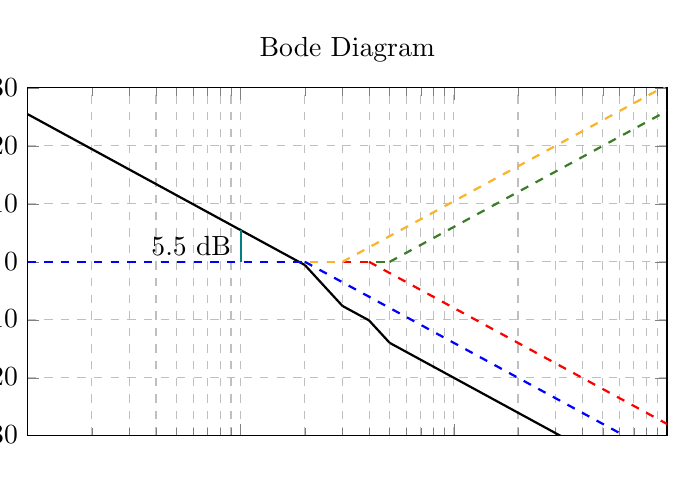
\begin{tikzpicture}[trim axis left,trim axis right]
			\begin{semilogxaxis}[title=Bode Diagram, ylabel=Gain, xmin=1e-1, xmax=1e2, ymin=-30, ymax=30, xticklabels={,,}, width=0.8\textwidth,height=6cm,ytick={-30,-20,-10,0,10,20,30},grid=both,grid style={dashed}];	
			\addplot[thick,domain=1e-1:2] {20*log10(15/8)-20*log10(x)};
			\addplot[thick,domain=2:3] {20*log10(15/8)-40*log10(x)+20*log10(2)};
			\addplot[thick,domain=3:4] {20*log10(15/8)-20*log10(x)+20*log10(2)-20*log10(3)};
			\addplot[thick,domain=4:5] {20*log10(15/8)-40*log10(x) +20*log10(2)-20*log10(3)+20*log10(4)};
			\addplot[thick,domain=5:1e2] {20*log10(15/8)-20*log10(x) +20*log10(2)-20*log10(3)+20*log10(4)-20*log10(5)};
			
			\addplot[teal,thick] coordinates {(1,5.5) (1,0)};
			\node[left] at (axis cs: 1,2.75) {5.5 dB};
			
			\addplot[dashed,thick,domain=1e-1:5,OliveGreen] {0};
			\addplot[dashed,thick,domain=1e-1:4,red] {0};
			\addplot[dashed,thick,domain=1e-1:3,Dandelion] {0};
			\addplot[dashed,thick,domain=1e-1:2,blue] {0};
			\addplot[dashed,thick,domain=2:1e2,blue] {20*log10(2)-20*log10(x)};		 
			\addplot[dashed,thick,domain=4:1e2,red] {20*log10(4)-20*log10(x)};	
			\addplot[dashed,thick,domain=3:1e2,Dandelion] {-20*log10(3)+20*log10(x)};		 
			\addplot[dashed,thick,domain=5:1e2,OliveGreen] {-20*log10(5)+20*log10(x)};	
			\end{semilogxaxis}
			\end{tikzpicture}
			
			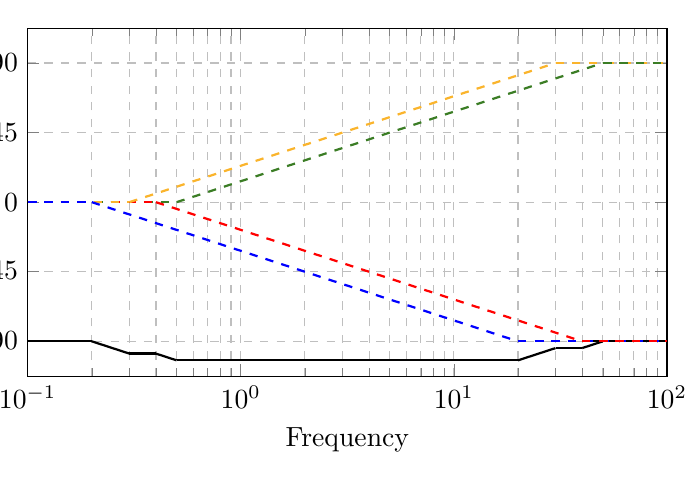
\begin{tikzpicture}[trim axis left,trim axis right]
			\begin{semilogxaxis}[xlabel=Frequency, ylabel=Phase, xmin=1e-1, xmax=1e2, ymin=-112.5, ymax=112.5, width=0.8\textwidth,height=6cm,ytick={-90,-45,0,45,90},grid=both,grid style={dashed}];
			
			\addplot[thick,domain=1e-1:0.2] {-90};
			\addplot[thick,domain=0.2:0.3] {-90-45*log10(x)+45*log10(0.2)};
			\addplot[thick,domain=0.3:0.4] {-90-0*log10(x)+45*log10(0.2)-45*log10(0.3)};
			\addplot[thick,domain=0.4:0.5] {-90-45*log10(x) +45*log10(0.2)-45*log10(0.3)+45*log10(0.4)};
			\addplot[thick,domain=0.5:20] {-90-0*log10(x) +45*log10(0.2)-45*log10(0.3)+45*log10(0.4)-45*log10(0.5)};
			\addplot[thick,domain=20:30] {-90+45*log10(x) +45*log10(0.2)-45*log10(0.3)+45*log10(0.4)-45*log10(0.5) -45*log10(20)};
			\addplot[thick,domain=30:40] {-90-0*log10(x) +45*log10(0.2)-45*log10(0.3)+45*log10(0.4)-45*log10(0.5) -45*log10(20)+45*log10(30)};
			\addplot[thick,domain=40:50] {-90+45*log10(x) +45*log10(0.2)-45*log10(0.3)+45*log10(0.4)-45*log10(0.5) -45*log10(20)+45*log10(30)-45*log10(40)};
			\addplot[thick,domain=40:1e2] {-90};
			
			\addplot[dashed,thick,domain=1e-1:0.5,OliveGreen] {0};
			\addplot[dashed,thick,domain=1e-1:0.4,red] {0};
			\addplot[dashed,thick,domain=1e-1:0.3,Dandelion] {0};
			\addplot[dashed,thick,domain=1e-1:0.2,blue] {0};
			\addplot[dashed,thick,domain=20:1e2,blue] {-90};
			\addplot[dashed,thick,domain=40:1e2,red] {-90};
			\addplot[dashed,thick,domain=0.2:20,blue] {-45*log10(x)+45*log10(0.2)};		 
			\addplot[dashed,thick,domain=0.4:40,red] {-45*log10(x)+45*log10(0.4)};		 
			\addplot[dashed,thick,domain=0.3:30,Dandelion] {45*log10(x)-45*log10(0.3)};			 
			\addplot[dashed,thick,domain=0.5:50,OliveGreen] {45*log10(x)-45*log10(0.5)};
			\addplot[dashed,thick,domain=30:1e2,Dandelion] {90};
			\addplot[dashed,thick,domain=50:1e2,OliveGreen] {90};
			
			\end{semilogxaxis}
			\end{tikzpicture}
		\end{center}
	\clearpage	
	\item Draw the Bode asymptote plot for 
	\[ G(s) = \dfrac{50}{s(0.2s+1)} \]
	\textbf{Solution:}
	\begin{itemize}
		\item 1 integrator, so start with $ -20 $dB/dec slope with 0dB at $ \omega=1 $ rad/s and $ -90^\circ $ phase.
		\item $ K=50 = 34 $ dB, so shift by 34dB (no change to phase plot).
		\item Pole at $ s=-5 $ (blue) add $ -20 $dbB/dec at $ \omega=5 $, and a $ -90^\circ $ shift from $ \omega=0.5 $ to $ \omega=50 $. (Or, adds $ -45^\circ $/dec at $ \omega=0.5 $ and $ +45^\circ $/dec at $ \omega=50 $.)
	\end{itemize}
	\begin{center}
		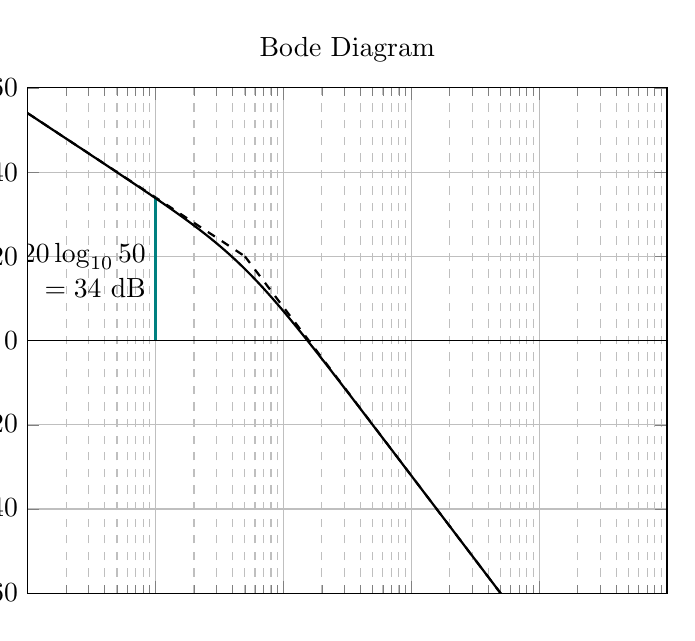
\begin{tikzpicture}[trim axis left,trim axis right]
		\begin{semilogxaxis}[title=Bode Diagram, ylabel=Gain, xmin=1e-1, xmax=1e4, ymin=-60, ymax=60, xticklabels={,,}, width=0.8\textwidth,height=8cm,ytick={-60,-40,-20,0,20,40,60},grid=both,minor grid style={dashed}];	
		
		\addplot[dashed,thick,domain=1e-1:5] {20*log10(50)-20*log10(x)};
		\addplot[dashed,thick,domain=5:1e4] {20*log10(50)-40*log10(x)+20*log10(5)};
		
		\addplot[teal,thick] coordinates {(1,0) (1,34 )};
		\node[left] at (axis cs: 1,20) {$ 20\logg50 $};
		\node[left] at (axis cs: 1,12.5) {$ =34 $ dB};
		
		\addplot[domain=1e-1:1e4] {0};
		
		\addplot[thick,domain=1e-1:1e4,samples=500] {20*log10( 50 ) - 20*log10( x ) - 20*log10( sqrt( 1 + (x/5)^2 ) )};
		
		\end{semilogxaxis}
		\end{tikzpicture}
		
		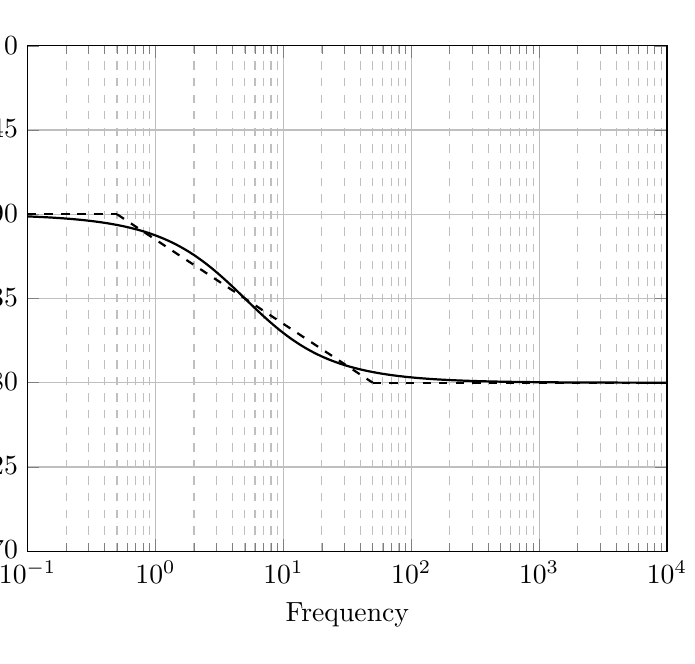
\begin{tikzpicture}[trim axis left,trim axis right]
		\begin{semilogxaxis}[xlabel=Frequency, ylabel=Phase, xmin=1e-1, xmax=1e4, ymin=-270, ymax=0, width=0.8\textwidth,height=8cm,ytick={0,-45,-90,-135,-180,-225,-270},grid=both,minor grid style={dashed}];
		
		\addplot[thick,dashed,domain=1e-1:0.5] {-90};
		\addplot[thick,dashed,domain=0.5:50] {-90-45*log10(x)+45*log10(0.5)};
		\addplot[thick,dashed,domain=50:1e4] {-180};
		
		\addplot[thick,domain=1e-1:1e4,samples=400] {-90 - atan(x/5)};
		
		\end{semilogxaxis}
		\end{tikzpicture}
	\end{center}
	\clearpage
	\item For the Bode diagram below, determine the transfer function.
	\begin{center}
		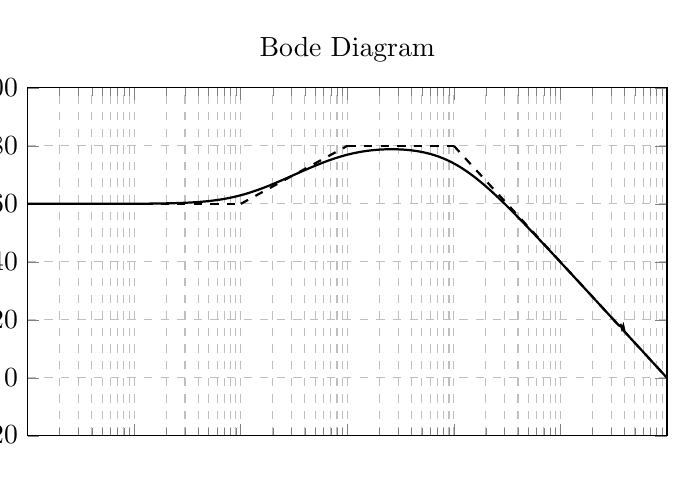
\begin{tikzpicture}[trim axis left,trim axis right]
		\begin{semilogxaxis}[title=Bode Diagram, ylabel=Gain, xmin=1e-2, xmax=1e4, ymin=-20, ymax=100, xticklabels={,,}, width=0.8\textwidth,height=6cm,ytick={-20,0,20,40,60,80,100},grid=both,grid style={dashed}];	
		\addplot[dashed,thick,domain=1e-2:1e0] {60};
		\addplot[dashed,thick,domain=1e0:1e1] {60+20*log10(x)};
		\addplot[dashed,thick,domain=1e1:1e2] {80};
		\addplot[dashed,thick,domain=1e2:1e4] {160-40*log10(x)};
		
		\addplot[thick,domain=1e-2:1e4,samples=500] {20*log10( 1000 * sqrt(1+(x)^2) / sqrt(1+(x/10)^2) / sqrt( 1 + (x/100)^2 )^2 )}; 
		
		\end{semilogxaxis}
		\end{tikzpicture}
		
		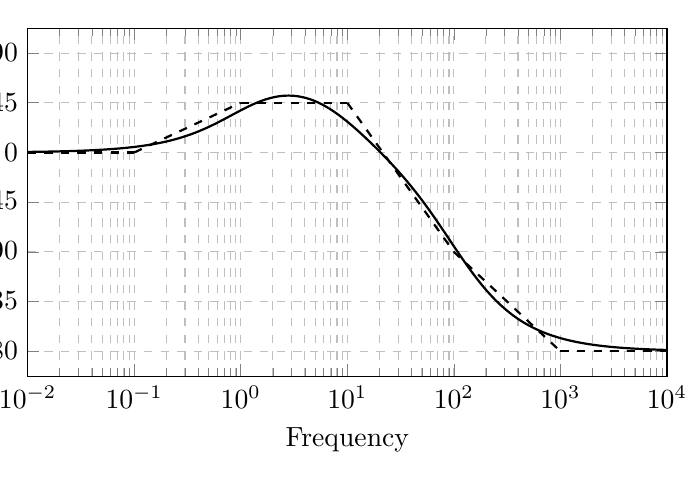
\begin{tikzpicture}[trim axis left,trim axis right]
		\begin{semilogxaxis}[xlabel=Frequency, ylabel=Phase, xmin=1e-2, xmax=1e4, ymin=-202.5, ymax=112.5, width=0.8\textwidth,height=6cm,ytick={-180,-135,-90,-45,0,45,90},grid=both,grid style={dashed}];
		
		\addplot[dashed,thick,domain=1e-1:1e0] {45+45*log10(x)};
		\addplot[dashed,thick,domain=1e0:1e1] {45};
		\addplot[dashed,thick,domain=1e1:1e2] {180-135*log10(x)};
		\addplot[dashed,thick,domain=1e2:1e3] {90-90*log10(x)};
		\addplot[dashed,thick,domain=1e3:1e4] {-180};
		\addplot[dashed,thick,domain=1e-2:1e-1] {0};
		
		\addplot[thick,domain=1e-2:1e4,samples=400] { atan(x) - atan(x/10) - 2*atan(x/100) }; 	
		
		\end{semilogxaxis}
		\end{tikzpicture}
	\end{center}
	
	\begin{itemize}
		\item 60dB magnitude as $ s\to 0 $: $ K=60dB=1000 $.
		\item +20dB/dec slope at $ \omega=1 $; +45$ ^\circ $/dec phase centered on $ \omega=1 $. Therefore, there is a zero at $ \omega=1 $.
		\item --20dB/dec slope at $ \omega=10 $; --45$ ^\circ $/dec phase centered on $ \omega=10 $. Therefore, there is a pole at $ \omega=10 $.
		\item --40dB/dec slope at $ \omega=100 $; --90$ ^\circ $/dec phase centered on $ \omega=100 $ and over 2 decades. Therefore, there are two poles at $ \omega=100 $.
		\[ \Rightarrow L(s) = \frac{1000\left(s+1\right)}{\left(\dfrac{s}{10}+1\right)\left(\dfrac{s}{100}+1\right)^2} \]
	\end{itemize}
	
\end{enumerate}


\end{document}

